%{{{ Formatierung

\documentclass[a4paper,10pt]{article}

\usepackage{physics_notetaking}

%%% dark red
%\definecolor{bg}{RGB}{60,47,47}
%\definecolor{fg}{RGB}{255,244,230}
%%% space grey
%\definecolor{bg}{RGB}{46,52,64}
%\definecolor{fg}{RGB}{216,222,233}
%%% purple
%\definecolor{bg}{RGB}{69,0,128}
%\definecolor{fg}{RGB}{237,237,222}
%\pagecolor{bg}
%\color{fg}

\newcommand{\td}{\,\text{d}}
\newcommand{\RN}[1]{\uppercase\expandafter{\romannumeral#1}}
\newcommand{\zz}{\mathrm{Z\kern-.3em\raise-0.5ex\hbox{Z} }}
\newcommand{\id}{1\kern-.258em1}

\newcommand\inlineeqno{\stepcounter{equation}\ {(\theequation)}}
\newcommand\inlineeqnoa{(\theequation.\text{a})}
\newcommand\inlineeqnob{(\theequation.\text{b})}
\newcommand\inlineeqnoc{(\theequation.\text{c})}

\newcommand\inlineeqnowo{\stepcounter{equation}\ {(\theequation)}}
\newcommand\inlineeqnowoa{\theequation.\text{a}}
\newcommand\inlineeqnowob{\theequation.\text{b}}
\newcommand\inlineeqnowoc{\theequation.\text{c}}

\renewcommand{\refname}{Source}
\renewcommand{\sfdefault}{phv}
%\renewcommand*\contentsname{Contents}

\newenvironment{Figure}
        {\par\medskip\noindent\minipage{\linewidth}}
        {\endminipage\par\medskip} % for multicols figures

\pagestyle{fancy}

\sloppy

\numberwithin{equation}{section}

%}}}

\begin{document}

%{{{ Titelseite

\begin{titlepage}
        \title{6 (2. Halbtag) $|$ Operationsverstärker}
        \author[1]{Angelo Brade\thanks{s72abrad@uni-bonn.de}}
        \author[1]{Jonas Wortmann\thanks{s02jwort@uni-bonn.de}}
        \affil{Rheinische Friedrich--Wilhemls Universität Bonn}
\end{titlepage}

\iffalse\title{}
\author{}\fi

\maketitle
\pagenumbering{gobble}

%}}}

\clearpage

%{{{ Inhaltsverzeichnis

\fancyhead[R]{\leftmark}
%\fancyhead[R]{\leftmark\\\rightmark}
\fancyhead[L]{\thepage}
\fancyfoot[C]{}

\tableofcontents

%}}}

\clearpage

%{{{

\pagenumbering{arabic}

\begin{multicols}{2}
        \sloppy

        \section{Introduction}
        In this experiment, 6 groups will constrcut 6 different circuits and connect them to one big circuit.
        The result will look like this.
        \begin{Figure}
                \centering
                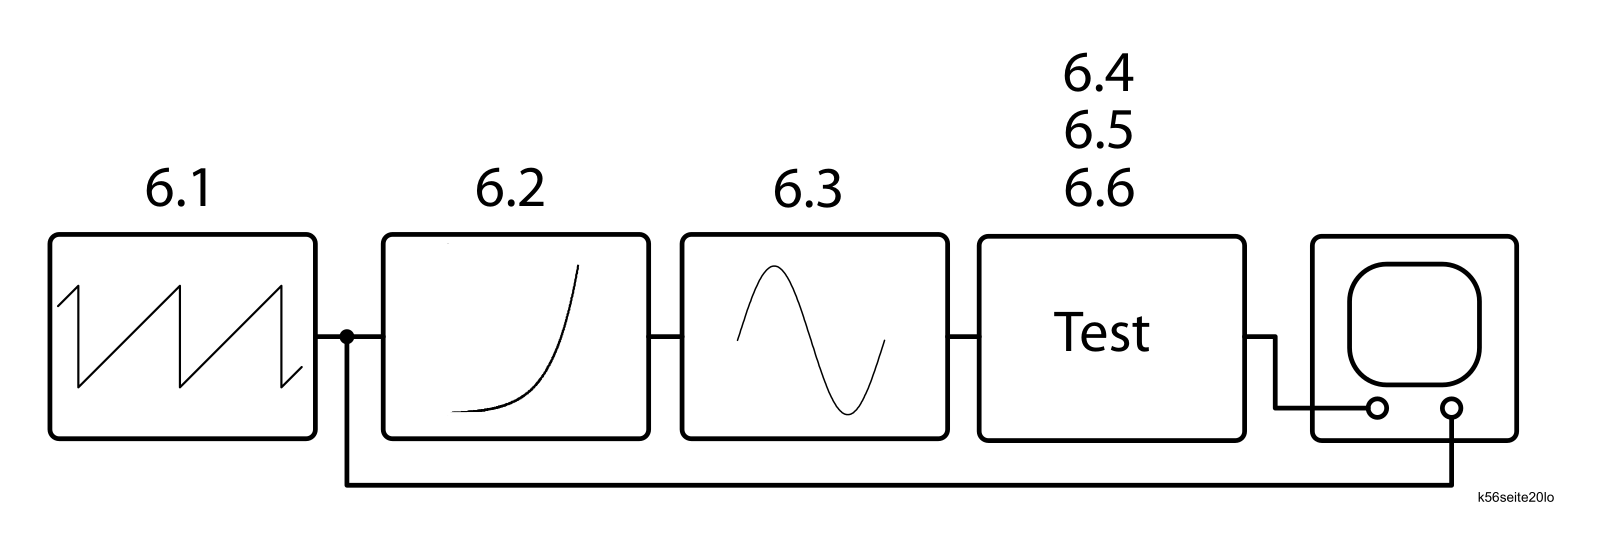
\includegraphics[width=0.7\textwidth]{result.png}
                \captionof{figure}{Circuit built from 6 individual smaller circuits; Abb. 6.14\cite{Praktikumsanleitung}}
        \end{Figure}
        \noindent This resulting circuit will show different usecases of the opamp, for example, demonstrate different configurations of high-- and lowpass filters as well as working as a resonanz amplifier.

        \section{Theory}
        The six different circtuis are
        \begin{enumerate}[label=\arabic*]
                \item Ramp generator: 
                        The ramp generator will input a ramp signal to the whole circuit.
                        The signal will be generated via the astable multivibrator.
                        This circuit utilises a condensator which charges and discharges in a certain time interval.
                \item Exponentiator: 
                        The inverting exponentiator has a very high input impedance compared to the non--inverting exponentiator, which makes it more suitable for this task. 
                        \begin{Figure}
                                \centering
                                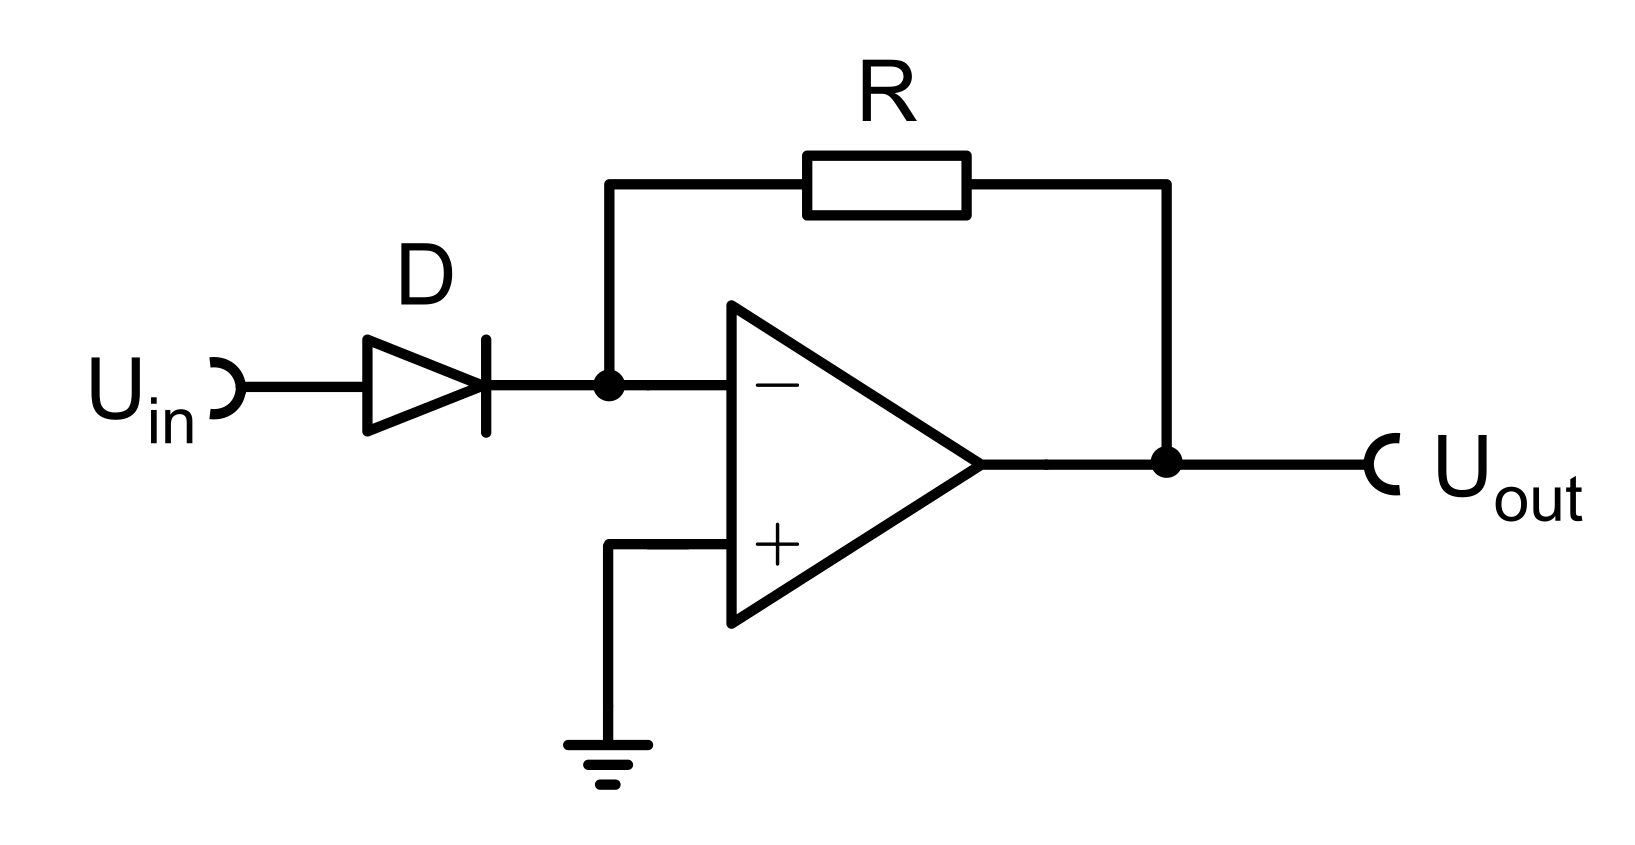
\includegraphics[width=0.6\textwidth]{inverting_exp.png}
                                \captionof{figure}{Inverting exponentiator; Abb.\ 6.4\cite{Praktikumsanleitung}}
                        \end{Figure}
                \item Voltage--frequency changer: 
                        This circuit proudces a triangle signal with constant amplitude by charging and discharging a capacitor.
                        The current is proportional to the input voltage.
                        \begin{Figure}
                                \centering
                                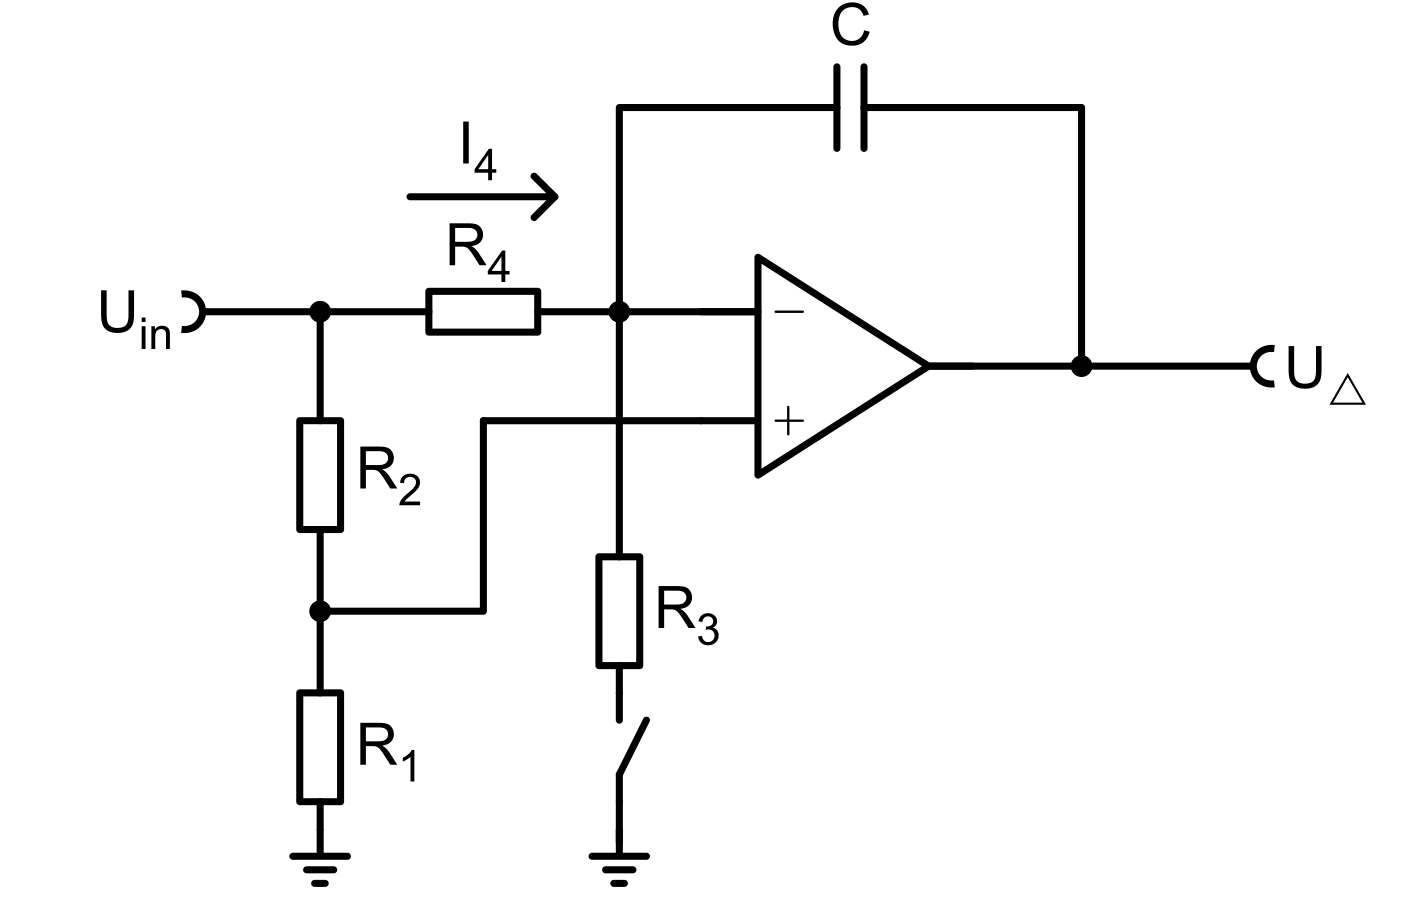
\includegraphics[width=0.6\textwidth]{reversible_integrator.png}
                                \captionof{figure}{Reversible integrator; Abb.\ 6.6\cite{Praktikumsanleitung}}
                        \end{Figure}
                        If the switch is open, the circuit behaves like a normal integrator and produces a constant decreasing output signal with current $I_4$.
                        If the switch is closed, a current across $R_3$ flows into the circuit which changes the sign of $I_4$ because both currents add.
                        This results in a constant increasing otuput signal.
                        For later use, the triangle signal will be modified into a sinosoidal signal.
                \item High-- and low--pass: 
                        For this circuit a third order low--pass is used, by connecting three low--passes in a row all seperated by an opamp with $\nu =1$.
                        \begin{Figure}
                                \centering
                                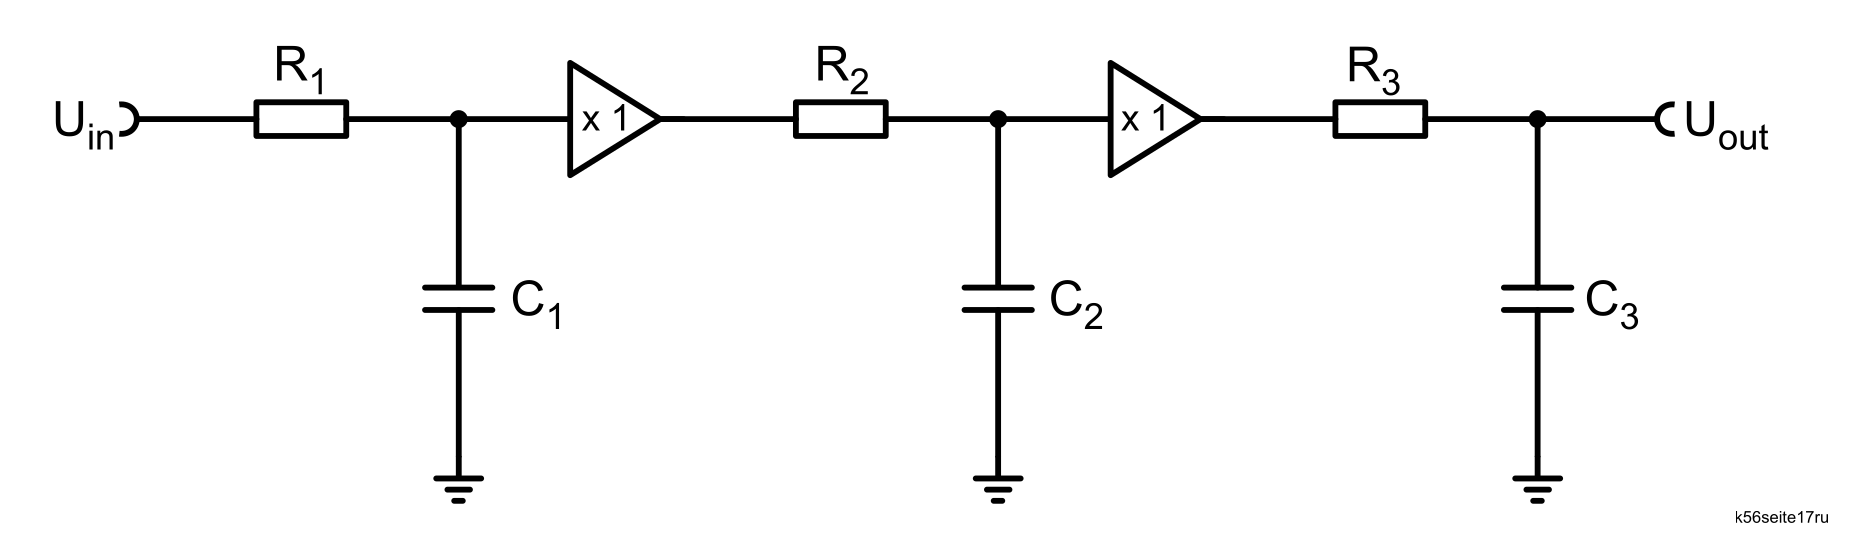
\includegraphics[width=0.6\textwidth]{lowpass_third_order.png}
                                \captionof{figure}{Third order low--pass; Abb.\ 6.10\cite{Praktikumsanleitung}}
                        \end{Figure}
                        In this configuration, their frequency response is multiplied.
                \item Band--elimination filter and resonance amplifier:
                        In this circuit a signal is sent through two low-- and high--passes connected in row.
                        The two outupt signals are then added via an opamp.
                        This results in a band--elimination filter.
                        \begin{Figure}
                                \centering
                                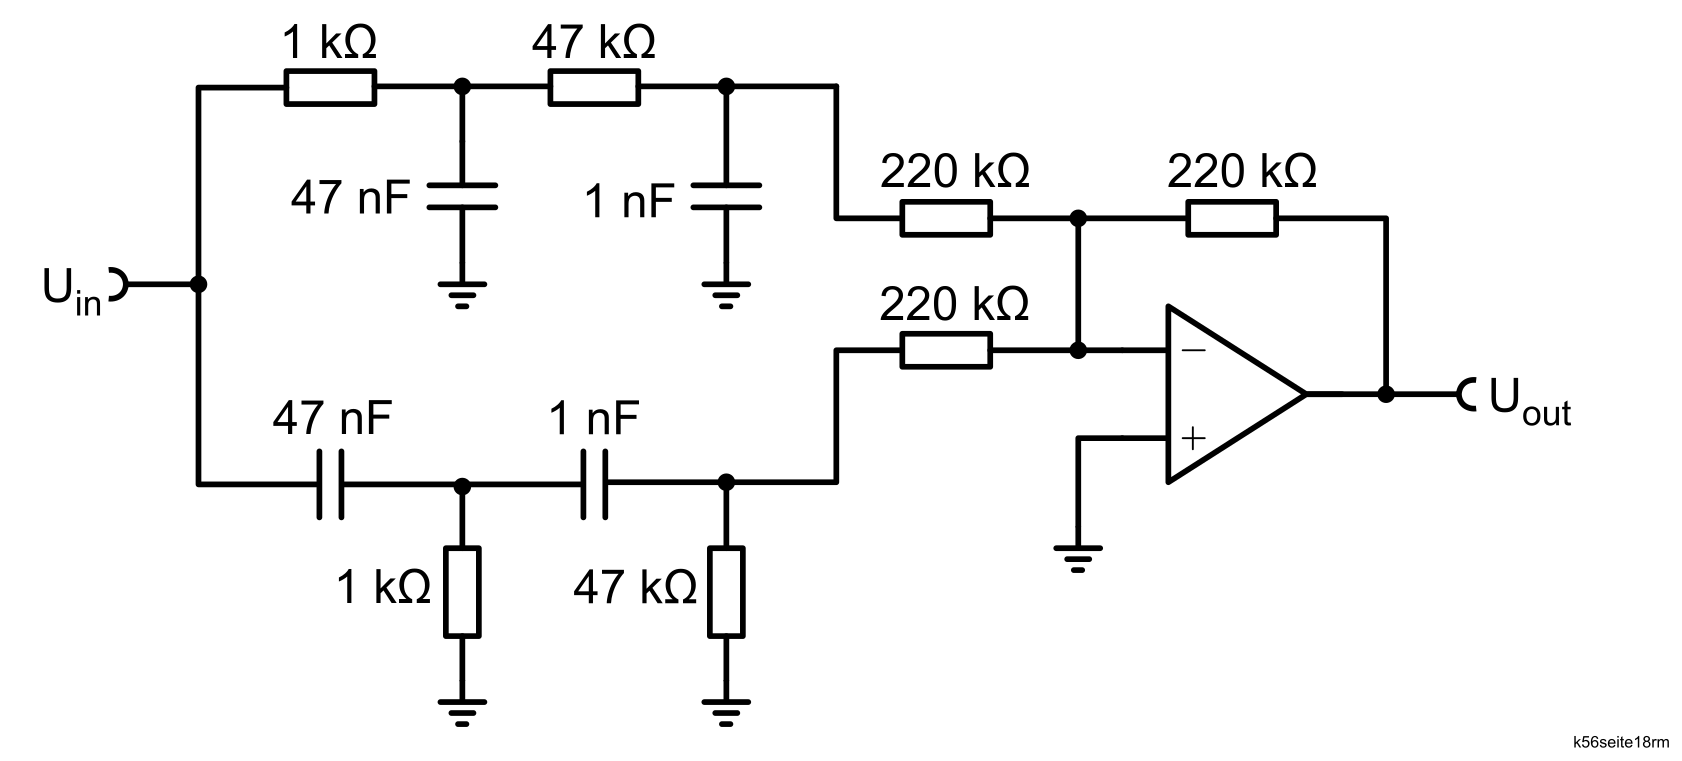
\includegraphics[width=0.6\textwidth]{band_elimination_filter.png}
                                \captionof{figure}{Band--elimination filter; Abb.\ 6.12\cite{Praktikumsanleitung}}
                        \end{Figure}
                \item Band--pass:
                        The last part is a band--pass.
                        \begin{Figure}
                                \centering
                                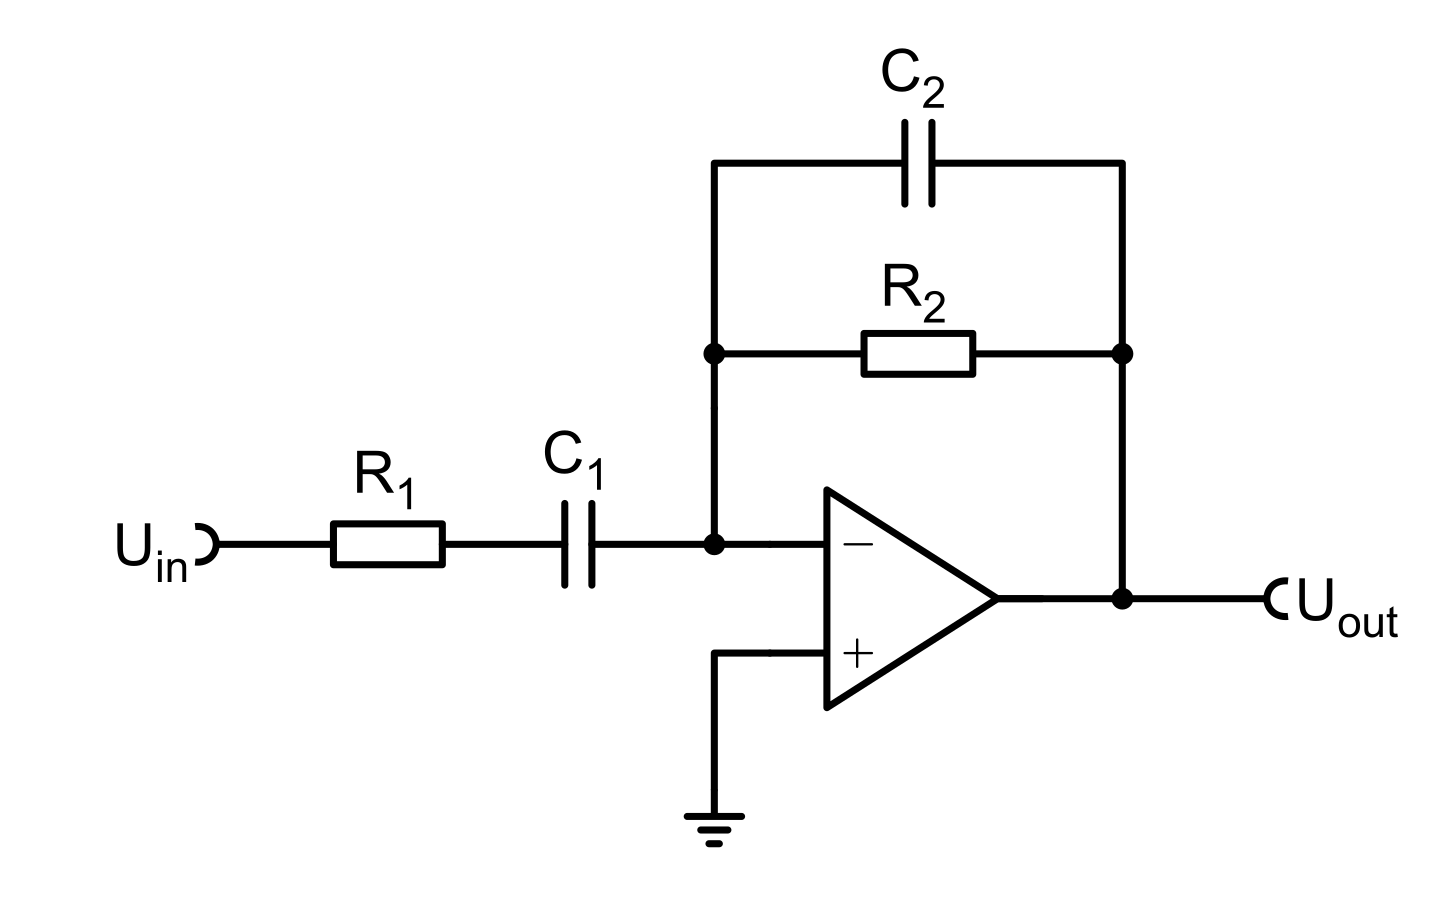
\includegraphics[width=0.6\textwidth]{bandpass.png}
                                \captionof{figure}{Band--pass; Abb.\ 6.13\cite{Praktikumsanleitung}}
                        \end{Figure}
        \end{enumerate}
        
        \clearpage
        \section{Analysis}


\end{multicols}

\clearpage
\listoffigures
\listoftables
\bibliographystyle{plain}
\bibliography{refs}

%}}}

\end{document}
